\section[玻尔的量子论]{玻尔的量子论}\label{sec:01.03}
% \makebox[5em][s]{} % 短题目拉间距
% \setlength{\mathindent}{9em} 本文标准公式缩进 
% \eqnormal % 恢复标准缩进

\textsf{1. 氢原子光谱}

19世纪后期,广泛进行了原子光谱的实验研究.1885年,巴尔末(Balmer)在氢原子光谱中发现了一个谱线系,其频率可以精确地表示成
\begin{equation}\label{eqn:01.03.01}
	\nu=\frac{c}{\lambda}=cR\bigg( \frac{1}{2^2}-\frac{1}{n^2} \bigg),\quad n=3,4,5,\cdots
\end{equation}
其中
\begin{equation*}
	R=\num{10967758.1} \si{m^{-1}} \text{(里德伯常数)}
\end{equation*}
后来又发现了其他谱线系.总的说,氢原子光谱全部谱线的频率可以归结成公式
\setlength{\mathindent}{6em}
\begin{equation}\label{eqn:01.03.02}
	\nu=\frac{c}{\lambda}=cR\bigg( \frac{1}{m^2}-\frac{1}{n^2} \bigg),\quad m<n \text{($m,n$为正整数)}
\end{equation}
\eqnormal
光谱公式虽然是经验公式,但是其精确度极高,为任何其他定量公式所不及.因此有理由相信,在这些公式后面一定隐藏着某种深刻的物理规律.

\textsf{2. 卢瑟福原子模型}

\begin{wrapfigure}[7]{r}{6em}
	\centering
	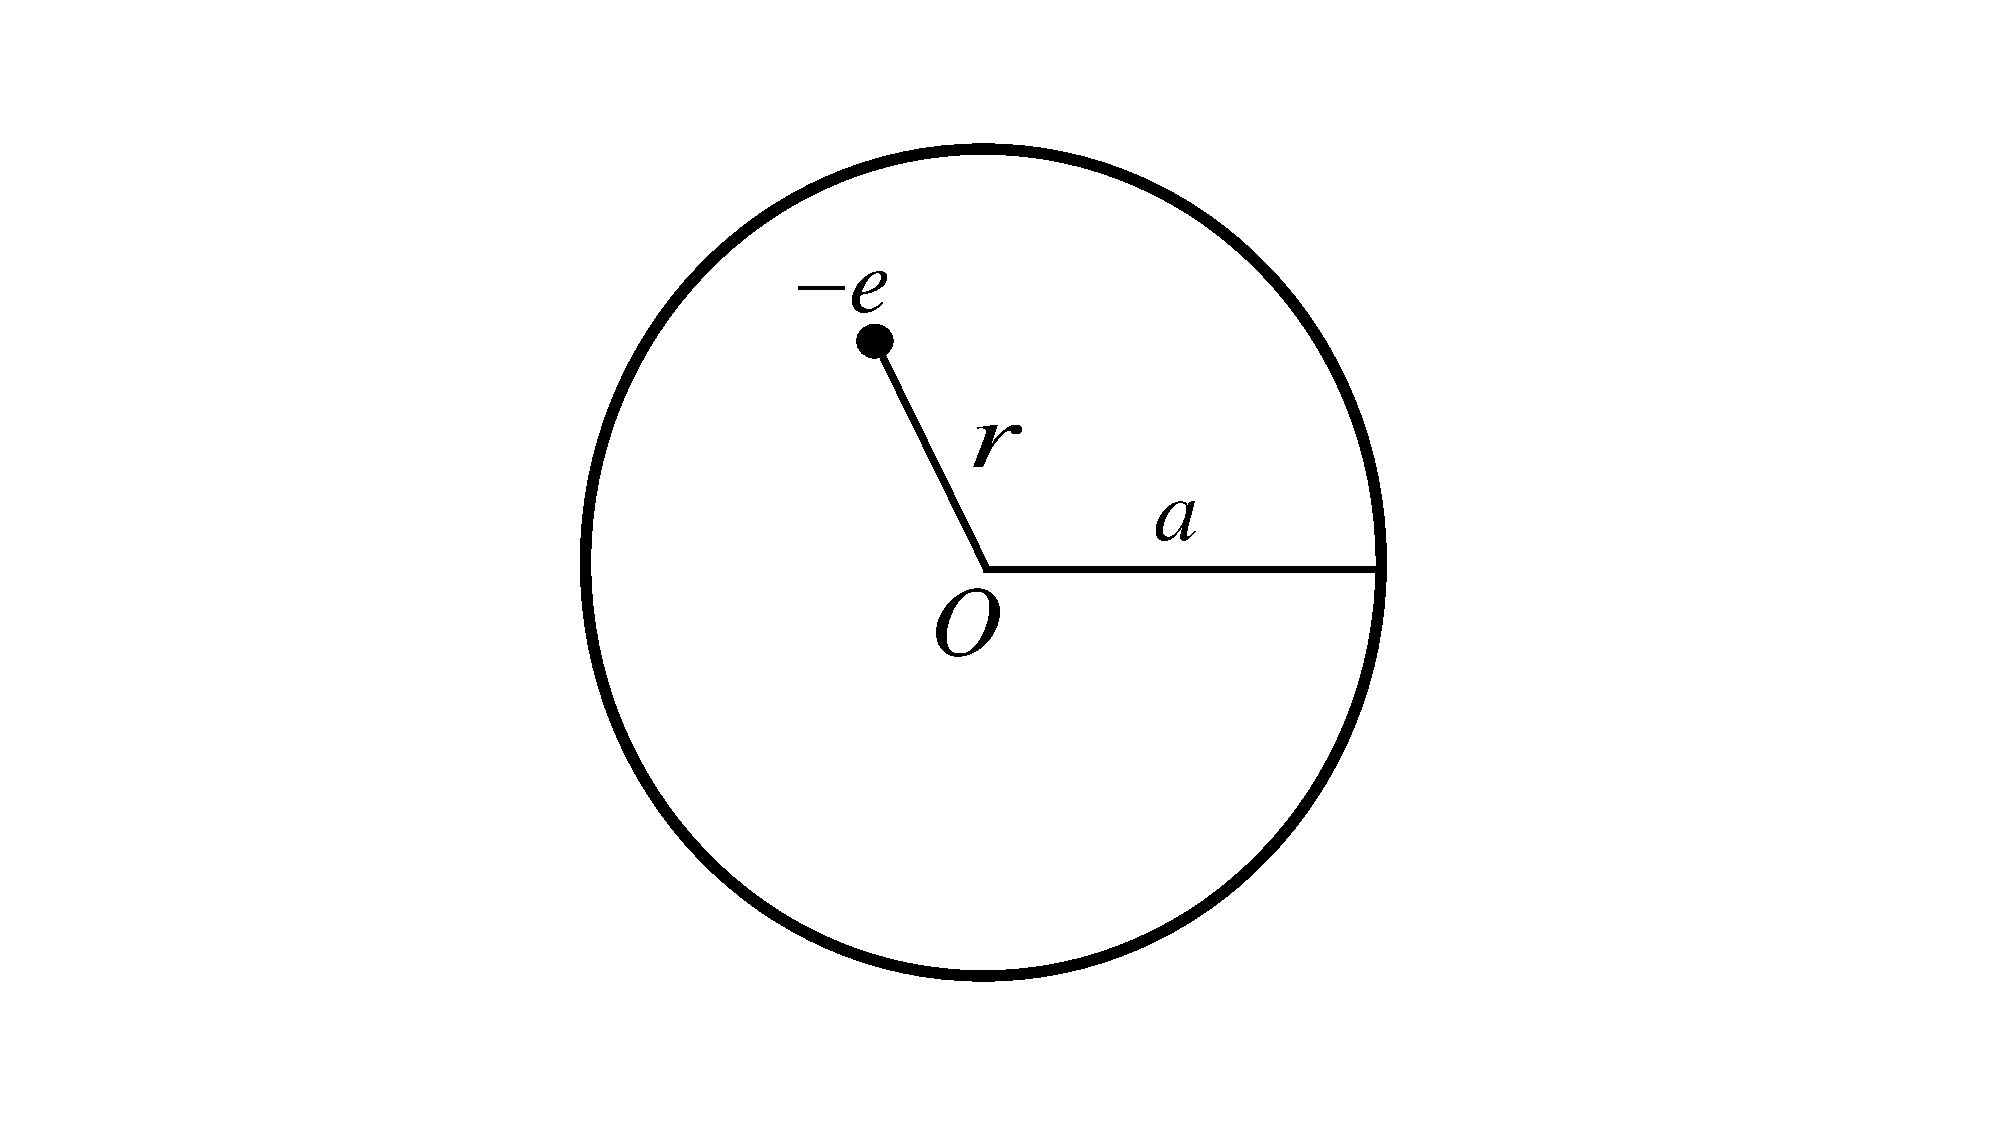
\includegraphics[width=2cm,clip]{QM file/figure/1-4}
	\caption{}
	\label{fig.1-4}
\end{wrapfigure}
1897年,汤姆孙(J.J.Tomson)用测量荷质比$\frac{e}{m_{e}}$的办法发现了电子.1903年,他顺理成章地提出了一种原子模型:原子的质量及正电荷均匀分布在球形体积中,球的半径即原子半径.电子(质量为$m_{e}$,远小于原子质量)在正电荷的库仑力作用下,可在原子内运动.按照汤姆孙原子模型,正常情况下电子停留在原子中心(球心),这时原子不发光.如因外力作用而使电子偏离了原子中心,正电荷对电子的库仑作用力将使电子在中心附近作简谐振动,从而向外辐射电磁波,即原子将发光.以单电子原子为例,如\ref{fig.1-4}所示,正电荷$Q=e$均匀分布在球内,电子(电荷$q=-e$)偏离球心时,库仑力为
\eqlong
\begin{equation}\label{eqn:01.03.03}
	\boldsymbol{F}=\-\frac{e^{2}}{4\pi\varepsilon_{0}}\bigg(\frac{r}{a} \bigg)^{3} \frac{r}{r^{3}}=-\frac{e^{2}}{4\pi\varepsilon_{0}}\frac{r}{a^{3}}
\end{equation}\eqnormal
今后,凡涉及库仑力问题,公式中$4\pi\varepsilon_{0}$一律省略不写.$\frac{e^{2}}{4\pi\varepsilon_{0}}$简记为$\e^{2}$.\eqref{eqn:01.03.03}式简写成
\eqshort
\begin{equation*}\label{eqn:01.03.03'}
	\boldsymbol{F}=-\frac{\e^{2}}{a^{3}} \boldsymbol{r} \tag{$1.3.3^{\prime}$}
\end{equation*}\eqnormal
库仑力表现为弹性力,因此电子将在球心附近作简谐运动,频率为
\eqlong
\begin{equation}\label{eqn:01.03.04}
	\nu=\frac{\omega}{2\pi}=\frac{1}{2\pi}\bigg(\frac{\e^2}{m_{e}a^3} \bigg)^{\frac{1}{2}}=\frac{1}{2\pi a}\bigg(\frac{\e^2}{m_{e}a^3} \bigg)^{\frac{1}{2}}
\end{equation}
电子振动时,将辐射出同样频率的电磁波,波长为
\begin{equation}\label{eqn:01.03.05}
	\lambda=\frac{c}{\nu}=2\pi ac\bigg(\frac{m_{e}a}{\e^2} \bigg)^{\frac{1}{2}}=2\pi a\bigg(\frac{a}{r_{e}} \bigg)^{\frac{1}{2}}
\end{equation}
其中为c光速,$r_{e}$为“经典电子半径”,
\begin{equation}\label{eqn:01.03.06}
	r_{e}=\frac{\e^2}{m_{e}c^{2}}=2.82\times10^{-15} \si{m}=2.82 \si{fm}
\end{equation}\eqnormal
如取原子半径$a\sim 0.1 \si{nm}=10^{-10} \si{m}$,求出
\begin{equation*}
	\lambda \sim 118 \si{nm},\quad \nu\sim 2.5\times10^{15} \si{s^{-1}}
\end{equation*}
属于紫外光区域.从数量级说,和原子光谱的范围大体相符.但是这种原子模型显然无法解释实验已经发现的氢原子光谱公式\eqref{eqn:01.03.02}.

汤姆孙原子模型终于被否定,是由于卢瑟福(Rutherford)的$\alpha$粒子对重元素的散射实验(1912)结果.

来自元素天然放射性的$\alpha$粒子,质量约为电子的7000倍,但比重元素的原子轻得多.因此在散射过程中,原子可以近似地当作是静止的.$\alpha$粒子的实验室动能约为几个$\si{MeV(10^{6} \si{eV})}$,远大于原子中电子的电离能(数量级$10\si{eV}$),因此当$\alpha$粒子与电子的距离接近到原子半径的量级时,即可使电子电离.只有原子中的正电荷才是使$\alpha$粒子发生散射的主要因素.

\begin{wrapfigure}[6]{r}{6em}
	\centering
	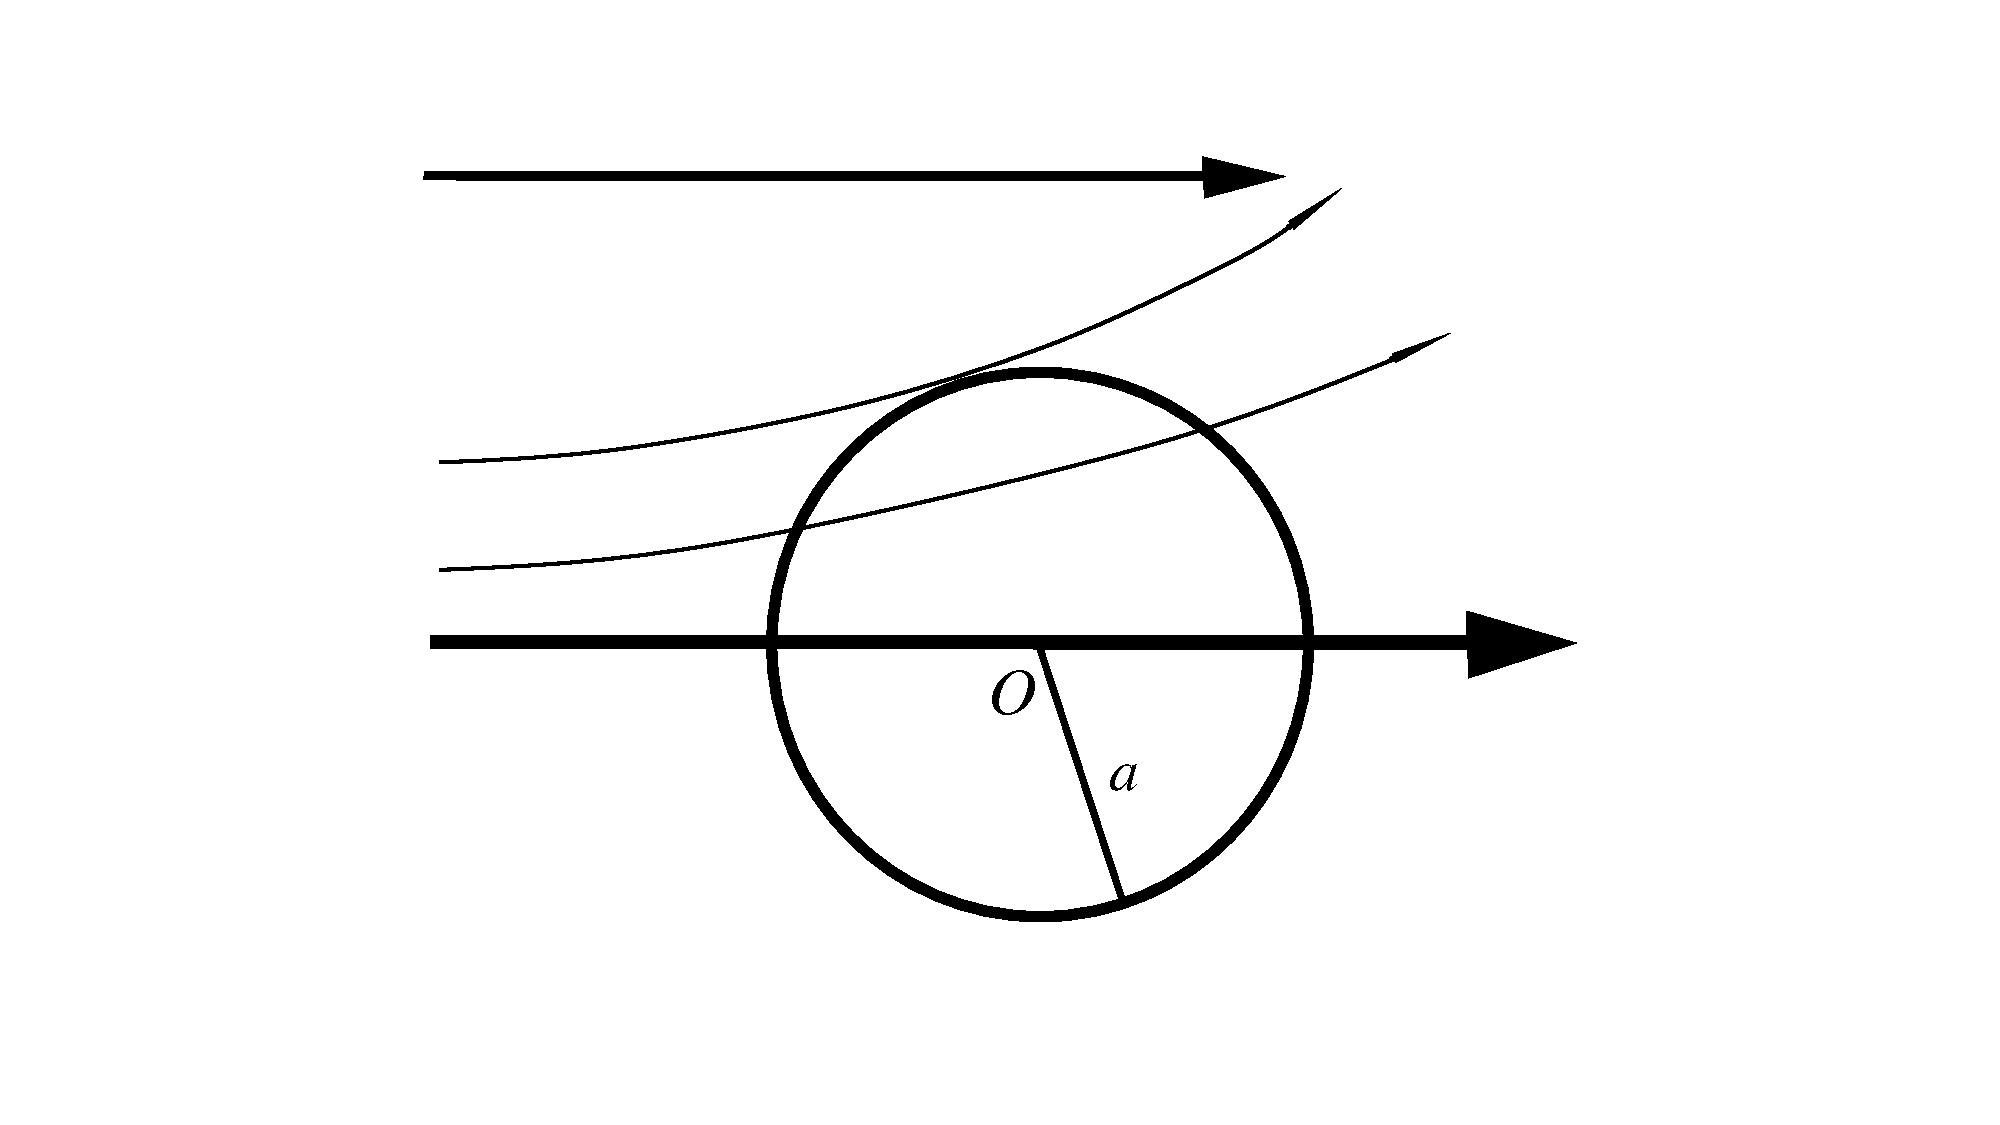
\includegraphics[width=2.5cm,clip]{QM file/figure/1-5}
	\caption{}
	\label{fig.1-5}
\end{wrapfigure}
令一束$\alpha$粒子以相同的初速度$v_{o}$射向一个汤姆孙原子,原子的正电荷($Q=Ze$,Z为原子序数)以库仑力作用于$\alpha$粒子,力的横向分量使$\alpha$粒子运动方向发生偏转.显然,在正电荷边缘掠过的$\alpha$粒子受到的横向力最大,偏转角也最大,如\ref{fig.1-5}所示.下面估算一下最大偏转角的量级.最大横向力约为
\begin{equation*}
	F_{\perp}\sim 2\e\cdot\frac{Z\e}{a^{2}}
\end{equation*}
有效作用时间约为$t\sim\frac{2a}{v_{0}}$,由此获得的横向动量约为
\begin{equation*}
	p_{\perp}\sim F_{\perp}\cdot t \sim\frac{4Z\e^{2}}{av_{0}}
\end{equation*}
因此,最大偏转角约为
\begin{equation}\label{eqn:01.03.07}
	\theta_{max}\sim \frac{p_{\perp}}{m_{a}v_{0}}\sim\frac{4Z\e^{2}}{m_{a}v_{0}^{2}a}=\frac{2Z\e^{2}/a}{E}
\end{equation}
其中$E=\frac{1}{2}m_{a}v_{0}^{2}$是$\alpha$粒子入射动能,$\frac{2Z\e^{2}}{a}$是最大静电势能.

以$\alpha$粒子被金原子(Z=79)散射为例,如取$a\sim 0.1\si{nm}$,$E\sim 5\si{MeV}$,则
\begin{gather}
	\frac{2Z\e^{2}}{a}\sim 2.3\times10^{-3} \si{MeV} \notag \\
	\theta_{max}\sim 4.6\times10^{-4} \notag
\end{gather}
而实验发现,最大偏转角可以超过$\frac{\pi}{2}$,甚至接近$\pi$.对实验结果的统计分析表明,这种大偏转角绝非多次散射的结果,而是由单次散射造成的.由此可知,原子中正电荷的分布半径应该远小于原子半径.为了解释大偏转角散射,原子中正电荷分布半径$R_{0}$应该满足关系:
\setlength{\mathindent}{12em}
\begin{equation}\label{eqn:01.03.08}
	\frac{2Z\e^{2}}{R_{0}} > E
\end{equation}
\eqnormal
这样,当$\alpha$粒子到达正电荷附近某个大于$R_{0}$的距离r时,静电势能$\frac{2Z\e^{2}}{r}$已经接近总能E,速度变小,在横向作用力的推动下,将形成大偏转角.如仍取Z=79,$E=5\si{MeV}$,\eqref{eqn:01.03.08}式给出$R<4.6\times10^{-14}\si{m}$,其量级稍大于原子核半径.

1912年,卢瑟福分析了$\alpha$粒子散射的实验结果后,提出了一种类似于太阳系的原子结构模型,即原子有核模型:原子的正电荷及绝大部分质量集中在很小的原子核(半径不超过10\si{fm})中,形成原子的坚实核心.电子在原子核的库仑力吸引下,环绕原子核运动,电子的轨道半径即原子半径.

在电磁辐射问题上,卢瑟福原子模型遭到了严重的困难,其程度较之汤姆孙模型有过之而无不及.按照经典力学,在原子核的库仑力场作用下,电子可以沿圆形或椭圆形轨道运动,原子核位于轨道的焦点处.电子运动的总机械能为负,并与圆的半径或椭圆的长半径成反比$\bigg(E=-\frac{Z\e^{2}}{2a} \bigg)$.按照经典电动力学,带电质点作加速运动时,将辐射电磁波.因此电子在运动过程中,将不断辐射电磁波,即发光,其频率等于电子的轨道频率及其倍频.由于对外辐射电磁波,电子运动的总能逐渐降低,轨道半径逐渐缩小,而运转频率则逐渐加快($\nu\propto a^{\frac{-3}{2}}$),最后电子将落入原子核中,即原子将崩溃.按照经典力学和电动力学的计算,如取初始原子半径$a\sim 0.1\si{nm}$,由于电磁辐射而造成原子崩溃的时间约为$10^{-10}\si{s}$.在此过程中,电子将辐射出各种频率的电磁波,频率呈现连续分布.

以上就是按照卢瑟福原子模型和经典物理理论描绘的原子辐射的情景,它显然与光谱公式\eqref{eqn:01.03.02}不符合,也与原子可以稳定存在这样一个经过多次实验证实的事实有着根本矛盾.

\textsf{3. 玻尔的量子论}

1913年,年仅28随的丹麦物理学家玻尔(N.Bohr)提出了原子结构的量子论.玻尔将卢瑟福原子模型和普朗克-爱因斯坦关于光辐射的量子论结合起来,扬弃了经典物理学的某些基本概念,而代之以一系列的量子假设.玻尔量子论的要点如下:

(1) 玻尔承认卢瑟福原子模型,但认为原子中的电子只能处于某些具有特定能量的状态(稳定轨道).如果没有外界作用,电子将始终沿着同一条稳定轨道运动,不辐射电磁波.也就是说,玻尔假定,对于电子的这些稳定状态,电动力学规律失效.

(2) 在外界作用下,如电子从一个稳定状态跃迁到另一个能量较低的稳定状态,则在此状态跃迁过程中,电子将发光(辐射电磁波),其频率为
\eqshort
\begin{equation}\label{eqn:01.03.09}
	\nu=\frac{E_{n}-E_{n^{\prime}}}{h}
\end{equation}\eqnormal
上式称为频率规则,$h$为普朗克常量.容易理解,\eqref{eqn:01.03.09}式是能量守恒定律和光量子概念的必然结论,但它与经典电动力学二理论存在根本概念上的矛盾.按照电动力学,电磁辐射频率应该等于电子当时的轨道运转频率,而\eqref{eqn:01.03.09}式则由跃迁前后两个状态的能量差决定.

(3) 在经典力学所允许的各个轨道中,只有符合量子化条件的轨道才是稳定轨道.玻尔当时只考虑了圆形轨道,提出的量子化条件为:轨道角动量的取值必须等于$h$(即$h/2\pi$)的整数倍,即
\begin{equation}\label{eqn:01.03.10}
	L=m_{e}vr=n\hbar,\quad n=1,2,3,\cdots
\end{equation}\eqlong
玻尔利用量子化条件\eqref{eqn:01.03.10}和频率规则\eqref{eqn:01.03.09},求出了氢原子中电子的稳定轨道的半径和能量,以及光谱频率,成功地解释了氢原子光谱公式\eqref{eqn:01.03.02}.

\begin{wrapfigure}[7]{r}{6em}
	\centering
	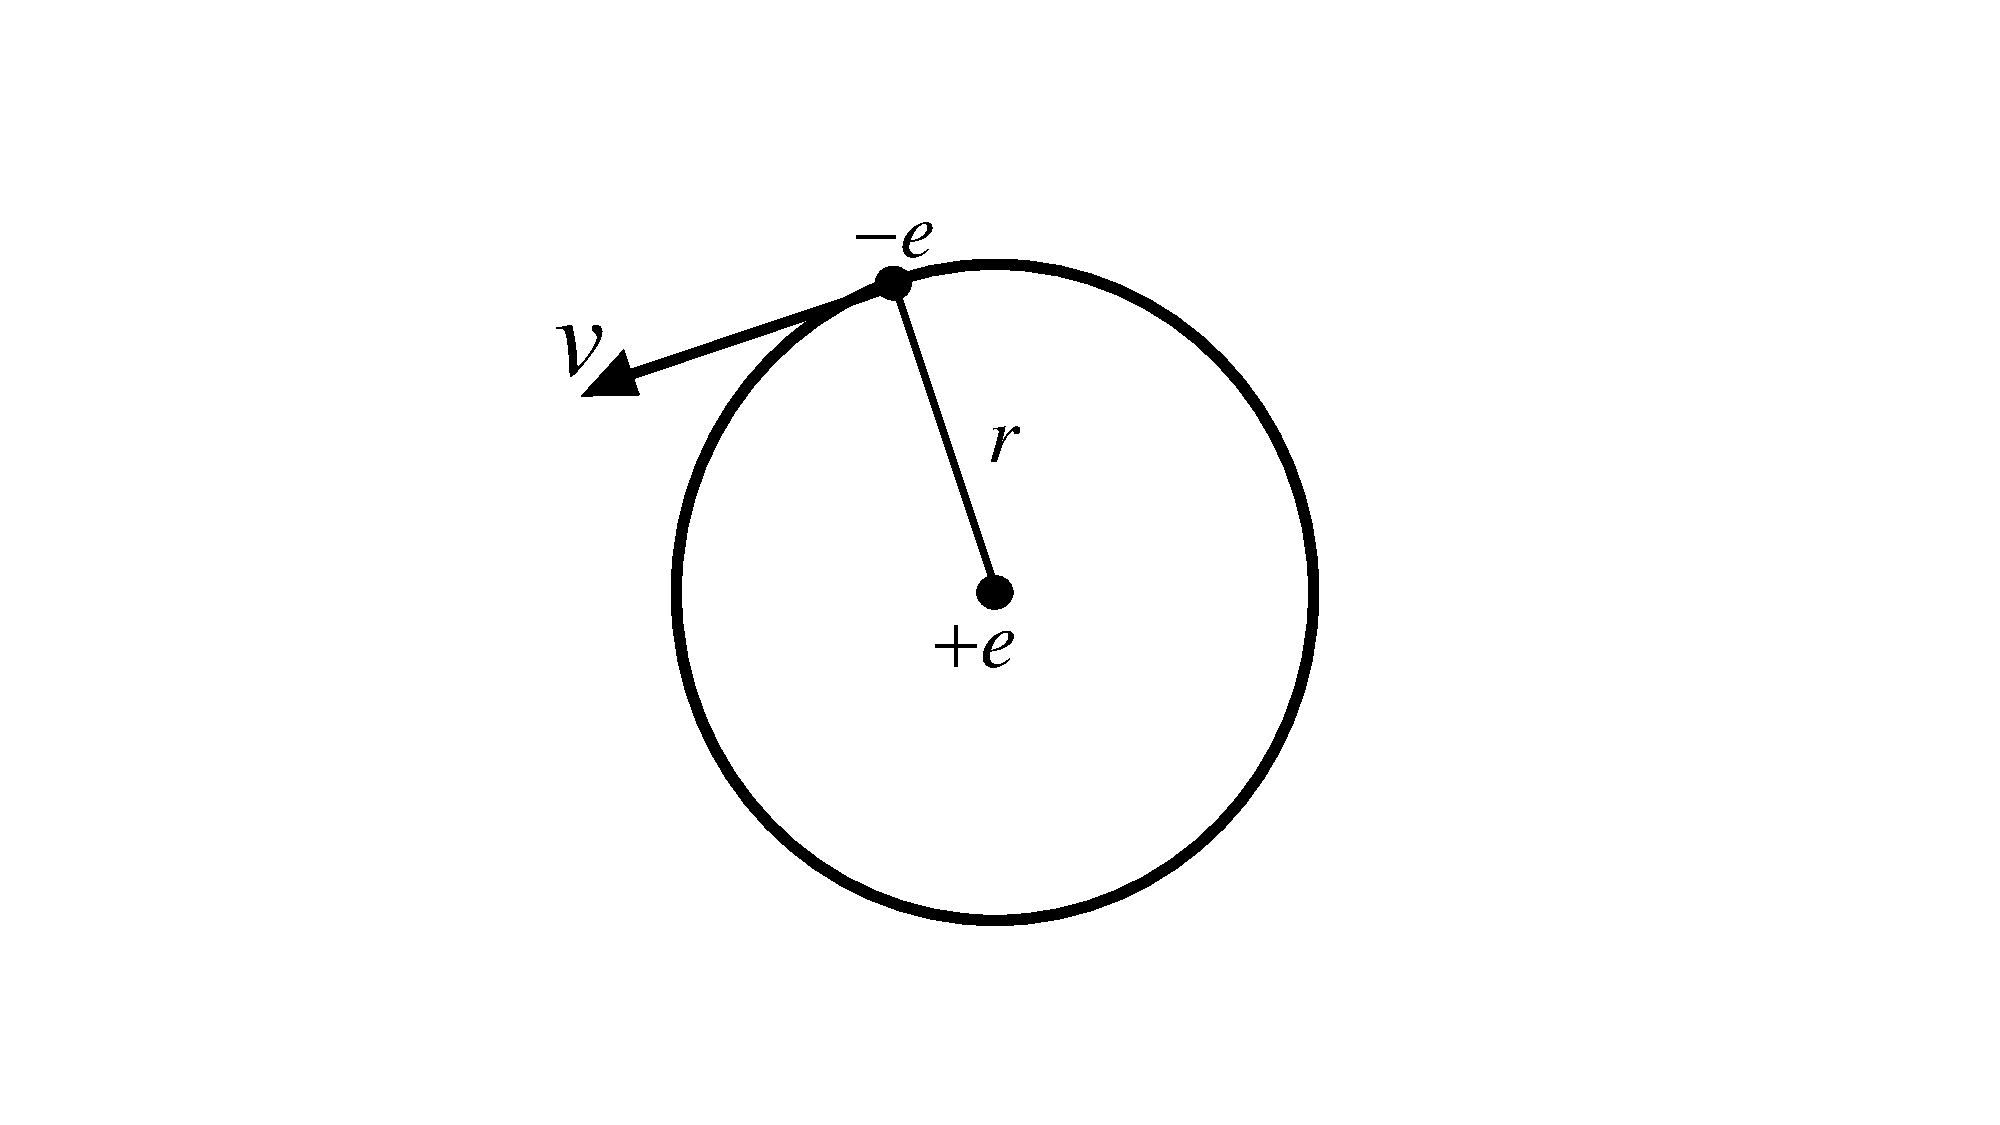
\includegraphics[width=2cm,clip]{QM file/figure/1-6}
	\caption{}
	\label{fig.1-6}
\end{wrapfigure}
后来,索末菲(Sommerfeld)将玻尔地量子化条件推广成为
\begin{equation}\label{eqn:01.03.11}
	\oint pdq =nh\quad n=1,2,3,\cdots
\end{equation}\eqshort
$p,q$为一对共轭地正则动量和坐标,$\oint$表示对运动的一个周期积分.推广后的量子化条件可以适用于任何周期性轨道,例如氢原子中电子的椭圆轨道.

玻尔认为,量子理论和经典物理理论之间并无不可逾越的鸿沟.量子理论概念适用于微观尺度,也适用于宏观尺度,经典理论仅适用于宏观尺度,在宏观尺度上,两种理论应该是一致的.这个观点成为对应原理.玻尔在20世纪20年代到各国宣讲他的量子理论时,强调对应原理是一个核心概念,而量子化条件则并不重要.下面我们根据对应原理对氢原子的能级和光谱试作分析.

考虑到圆轨道\ref{fig.1-6},电子的轨道半径r,速率v和角频率(角速度)$\omega$间的关系是
\begin{equation}\label{eqn:01.03.12}
	v=r\omega
\end{equation}
\eqnormal
原子核(电荷e)对电子的库伦吸引力就是圆周运动的向心力,
\begin{equation*}
	\frac{\e^{2}}{r^{2}}=m_{e}\frac{v^{2}}{r}=m_{e}r\omega^{2}
\end{equation*}\eqshort
因此
\begin{equation}\label{eqn:01.03.13}
	r^{3}\omega^{2}=\frac{\e^{2}}{m_{e}}
\end{equation}\eqnormal
电子运动的总能为
\begin{equation*}
	E=\frac{1}{2}m_{e}v^{2}-\frac{\e^{2}}{r}=\frac{1}{2}m_{e}r^{2}\omega^{2}-\frac{\e^{2}}{r}
\end{equation*}\eqshort
利用\eqref{eqn:01.03.13}式,得到
\begin{equation}\label{eqn:01.03.14}
	E=-\frac{\e^{2}}{2r}
\end{equation}\eqnormal
或
\begin{equation}\label{eqn:01.03.15}
	\omega=\bigg(\frac{8}{m_{e} \e^{4}}\bigg)^{\frac{1}{2}}(-E)^{\frac{3}{2}}
\end{equation}
\eqref{eqn:01.03.13}至\eqref{eqn:01.03.13}式适用于任何一条圆形轨道.以$n=1,2,3,\cdots$表示稳定轨道的序号,相应的$r,E,\omega$记为$r_{n},E_{n},\omega_{n}$,并规定$r_{n}$的编号次序为$r_1 < r_2 < r_3<\cdots$,当n不断增大,$r_{n}\rightarrow\infty$,$E_{n}\rightarrow 0^{-}$,所以$n\gg 1$相当于宏观尺度.

当电子由能级$E_{n}$跃迁到$E_{n-1}$,按照频率规则,发光角频率为
\begin{equation}\label{eqn:01.03.16}
	\omega=2\pi v=\frac{E_{n}-E_{n-1}}{\hbar}
\end{equation}
而按照电动力学,发光频率等于轨道运转频率,即$\omega_{n}$.按照对应原理,在$n\gg 1$时,$\omega$应该趋于$\omega_{n}$,即
\begin{equation}\label{eqn:01.03.17}
	E_{n}- E_{n-1}=\hbar\omega\rightarrow\hbar\omega_{n}
\end{equation}
亦即
\begin{equation}\label{eqn:01.03.18}
	E_{n}- E_{n-1}\rightarrow \bigg(\frac{8\hbar^{2}}{m_{e}\e^{4}}\bigg)^{\frac{1}{2}} (-E_{n})^{\frac{3}{2}},\quad n\gg 1
\end{equation}
$n\gg 1$时,n的变化($\Delta n=1$)远小于n本身,可以当作连续变化,因此
\begin{equation*}
	E_{n}- E_{n-1}=\Delta E_{n}
	=\frac{\Delta E_{n}}{\Delta n}\rightarrow\frac{dE_{n}}{dn}
\end{equation*}
\eqref{eqn:01.03.18}式可当作微分方程:
\begin{equation*}\label{eqn:01.03.18'}
	 \frac{dE_{n}}{dn}=
	 \bigg(\frac{8\hbar^{2}}{m_{e}\e^{4}}\bigg)^{\frac{1}{2}}(-E_{n})^{\frac{3}{2}},
	 \quad n\gg1		\tag{$1.3.18^{\prime}$}
\end{equation*}
容易解出
\begin{equation}\label{eqn:01.03.19}
	E_{n}=-\frac{1}{2n^{2}}\frac{m_{e}\e^{4}}{\hbar^{2}}=-\frac{1}{2n^{2}}\frac{\e^{2}}{a_{0}}
\end{equation}
再利用\eqref{eqn:01.03.14}式,得到
\begin{equation}\label{eqn:01.03.20}
	r_{n}=-\frac{\e^{2}}{2E_{n}}=n^{2}\frac{\hbar^{2}}{m_{e}\e^{2}}=n^{2}a_{0}
\end{equation}
其中$a_{o}=\frac{\hbar^{2}}{m_{e}\e^{2}}$为玻尔半径,即氢原子基态(n=1)半径.\eqref{eqn:01.03.19}、\eqref{eqn:01.03.20}式是在条件$n\gg 1$下得到的,如果认为这些结果也适用于n较小的情况,则它们就是氢原子能级和轨道半径的量子化公式.

以L表示轨道角动量,利用\eqref{eqn:01.03.13}及\eqref{eqn:01.03.20}式,容易得到
\begin{equation*}
	L^{2}=(m_{e}vr^{2})^{2}=m_{e}^{2}\omega^{2}r^{4}=m_{e}^{2}\frac{\e^{2}}{m_{e}}n^{2}\frac{\hbar^{2}}{m_{e}\e^{2}}=n^{2}\hbar^{2}
\end{equation*}
亦即
\begin{equation*}
	L=n\hbar,\quad n=1,2,3,\cdots
\end{equation*}
这正是量子化条件\eqref{eqn:01.03.10}.

当电子由能级跃迁但,按照频率规则\eqref{eqn:01.03.09},放光频率为
\begin{equation}\label{eqn:01.03.21}
	\nu_{nm}=\frac{E_{n}-E_{m}}{h}=2\pi^{2}\frac{m_{e}\e^{4}}{h^{3}}\bigg(\frac{1}{m^{2}} -\frac{1}{n^{2}}\bigg)
\end{equation}
和经验公式\eqref{eqn:01.03.02}比较,二者一致,并得里德伯(Rydberg)常数的结构式:
\begin{equation}\label{eqn:01.03.22}
	R=\frac{2\pi^{2}m_{e}\e^{4}}{ch^{3}}=\frac{m_{e}\e^{4}}{4\pi c\hbar^{3}}
\end{equation}
以各基本常数之值代入上式,得到R的理论值为$R=\num{109737}\si{cm^{-1}}$.严格地说,氢原子问题是二体问题,求电子能级时应该用折合质量$\mu=\frac{m_{e}m_{p}}{m_{e}+m_{p}}$代替以上计算中地电子质量$m_{e}$,这样得到的氢原子光谱里德伯常数理论值为
\begin{equation}\label{eqn:01.03.23}
	R_{H}=\frac{2\pi^{2}\mu \e^{4}}{ch^{3}}=\num{109677} \si{cm^{-1}}
\end{equation}
和实验值符合得极好.

\example 对于氢原子的第n个玻尔圆形轨道,求电子运行速度.

\solution 根据量子化条件\eqref{eqn:01.03.10}及轨道半径公式\eqref{eqn:01.03.20},易得速度公式:
\begin{equation*}
	v=\frac{n\hbar}{m_{e}r_{n}}=\frac{\hbar}{nm_{e}a_{0}}=\frac{\e^{2}}{n\hbar}=\frac{c}{n}\frac{\e^{2}}{\hbar c}
\end{equation*}\eqshort
其中$\frac{\e^{2}}{\hbar c}=\frac{1}{137}$,所以
\begin{equation}\label{eqn:01.03.24}
	v=\frac{c}{137}\cdot\frac{1}{n}
\end{equation}\eqnormal
按数量级而言,$v$约为光速的几百分之一,约为$10^{6}\si{m/s}$.
